% Poses calculadas nos dois exemplos da cinemática inversa (plano do braço); unidades em cm
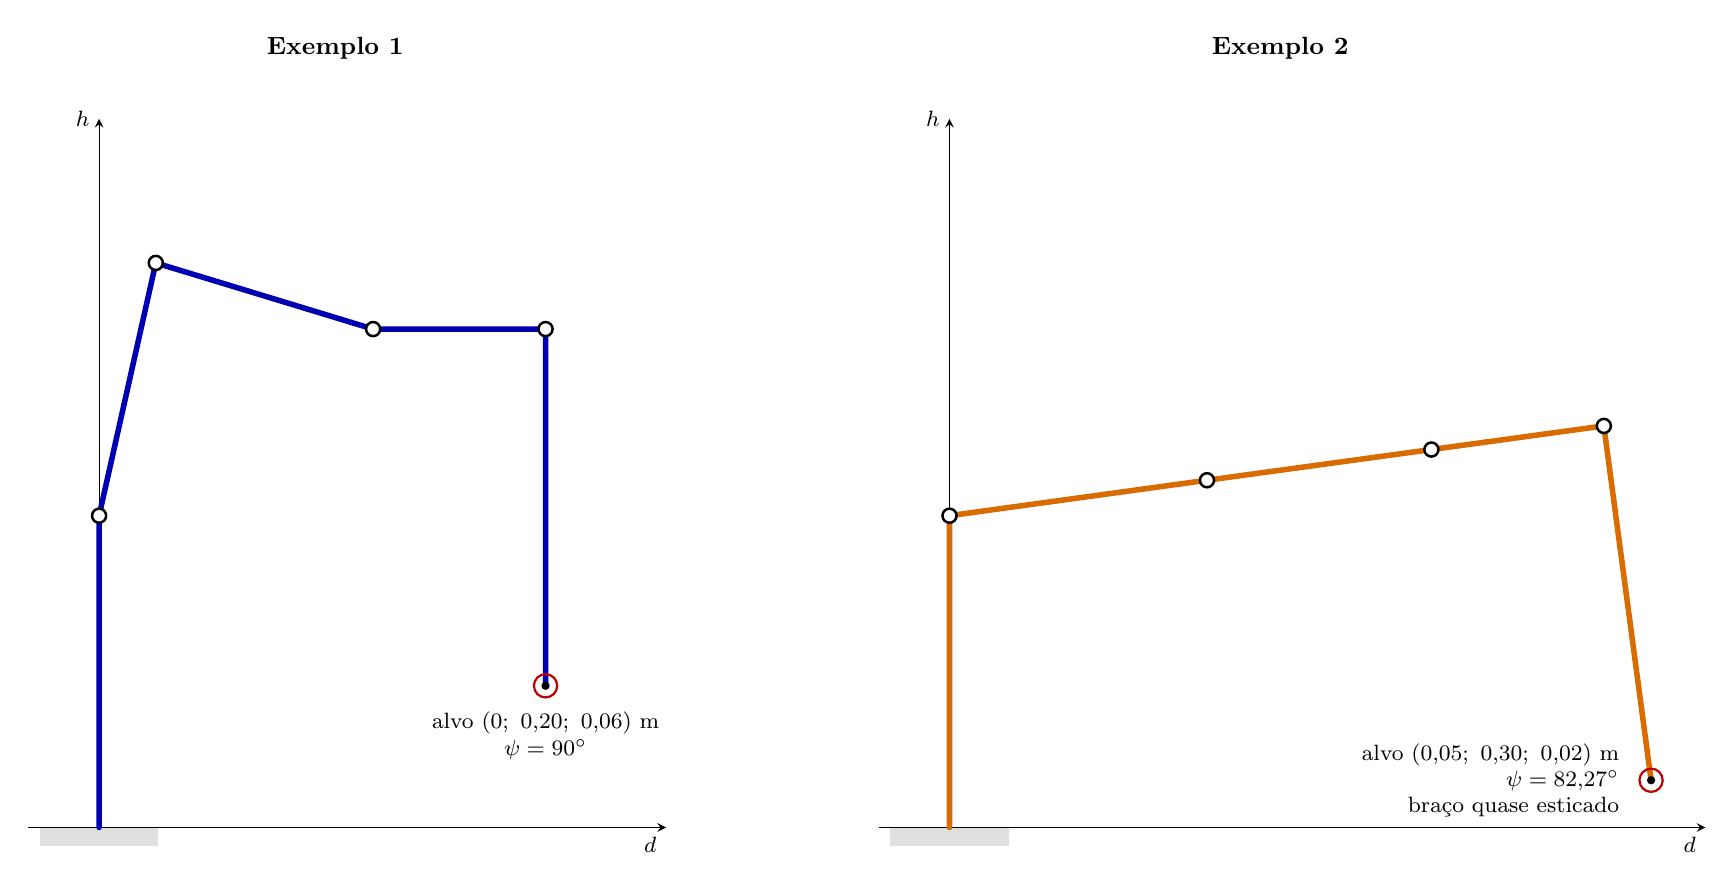
\begin{tikzpicture}[scale=0.3, >=stealth,
    elo/.style={line width=2pt, line cap=round},
    junta/.style={circle, draw, fill=white, line width=0.9pt, inner sep=1.8pt},
    cota/.style={gray!70!black, thin},
    ang/.style={->, thin},
    every node/.style={font=\footnotesize}]

  \draw[->, thin] (-3,0) -- (24,0) node[below left] {$d$};
  \draw[->, thin] (0,0) -- (0,30) node[left] {$h$};
  \fill[gray!25] (-2.5,-0.8) rectangle (2.5,0.0);
  \draw[elo, blue!70!black] (0.0,0.0) -- (0.0,13.2) -- (2.4,23.9) -- (11.6,21.1) -- (18.9,21.1) -- (18.9,6.0);
  \node[junta] at (0.0,13.2) {};
  \node[junta] at (2.4,23.9) {};
  \node[junta] at (11.6,21.1) {};
  \node[junta] at (18.9,21.1) {};
  \fill (18.9,6.0) circle (5pt);
  \draw[red!75!black, thick] (18.9,6.0) circle (14pt);
  \node[below=6pt, align=center] at (18.9,6.0) {alvo $(0;\ 0{,}20;\ 0{,}06)$ m\\$\psi = 90^\circ$};
  \node[font=\small\bfseries] at (10,33) {Exemplo 1};
  \draw[->, thin] (33,0) -- (68,0) node[below left] {$d$};
  \draw[->, thin] (36,0) -- (36,30) node[left] {$h$};
  \fill[gray!25] (33.5,-0.8) rectangle (38.5,0.0);
  \draw[elo, orange!85!black] (36.0,0.0) -- (36.0,13.2) -- (46.9,14.7) -- (56.4,16.0) -- (63.7,17.0) -- (65.7,2.0);
  \node[junta] at (36.0,13.2) {};
  \node[junta] at (46.9,14.7) {};
  \node[junta] at (56.4,16.0) {};
  \node[junta] at (63.7,17.0) {};
  \fill (65.7,2.0) circle (5pt);
  \draw[red!75!black, thick] (65.7,2.0) circle (14pt);
  \node[left=8pt, align=right] at (65.7,2.0) {alvo $(0{,}05;\ 0{,}30;\ 0{,}02)$ m\\$\psi = 82{,}27^\circ$\\braço quase esticado};
  \node[font=\small\bfseries] at (50,33) {Exemplo 2};
\end{tikzpicture}